\section{Pianificazione}
Alla luce delle scadenze presentate nella \hyperlink{scadenze}{sottosezione 1.5}, la pianificazione di progetto viene suddivisa nelle seguenti fasi:
\begin{enumerate}
	\item \textbf{Analisi};
	\item \textbf{Consolidamento dei requisiti};
	\item \textbf{Progettazione architetturale};
	\item \textbf{Progettazione di dettaglio e codifica};
	\item \textbf{Validazione e collaudo}.
\end{enumerate}
Ogni fase viene suddivisa in attività che verranno realizzate durante il 
periodo stabilito per la fase stessa. 
\subsection{Analisi}
\textit{Periodo: dal 2018-11-16 al 2019-01-14}\\
L'inizio del periodo di questa fase coincide con la data di formazione del 
gruppo e la fine coincide con la data ultima per la consegna dei documenti relativi alla 
revisione dei requisiti. Questa fase è stata scomposta nelle seguenti sotto attività:
\begin{itemize}
	\item \textbf{Individuazione degli strumenti}: questa attività consiste nel 
	determinare quali strumenti il gruppo deve utilizzare per la comunicazione, per 
la stesura dei documenti e per il versionamento, lo sviluppo e la verifica del 
software; 
	\item \textbf{Norme di progetto}: sono definite tutte le regole utili per lo svolgimento del progetto, relative al prodotto da realizzare e ai processi da adottare. Il documento Norme di Progetto viene redatto dall'\textit{Amministratore} per conto del \textit{Responsabile di progetto};
	\item \textbf{Studio di fattibilità}: in questa attività gli \textit{Analisti} effettuano uno studio sommario dei capitolati in modo da determinare quale di essi verrà scelto. Questa attività è da considerarsi bloccante per l'attività di Analisi dei requisiti;
	\item \textbf{Analisi dei requisiti}: durante questa attività vengono 
	identificati ed analizzati i requisiti del capitolato scelto nell'attività 
	di studio di fattibilità e il relativo documento viene composto dagli \textit{Analisti};
	\item \textbf{Piano di progetto}: il \textit{Responsabile} pianifica il 
	lavoro del gruppo \textit{8Lab Solutions}, inteso come suddivisione di compiti, 
	risorse e attività. Inoltre viene calcolato il preventivo per la realizzazione 
	del progetto. Questa attività comporta anche la stesura 
	del documento Piano di Progetto;
	\item \textbf{Piano di qualifica}: in questa attività si individuano le 
	metodologie attraverso le quali si garantisce la qualità del prodotto. A supporto di ciò viene redatto il documento Piano di Qualifica da parte dell'\textit{Amministratore} e per la parte programmatica dal \textit{Progettista}; 
	\item \textbf{Glossario}: tutti i termini che possono risultare ambigui vengono individuati e definiti nel documento Glossario, che viene redatto durante tutta la fase di analisi dei requisiti.
\end{itemize}

\begin{figure}[H]
	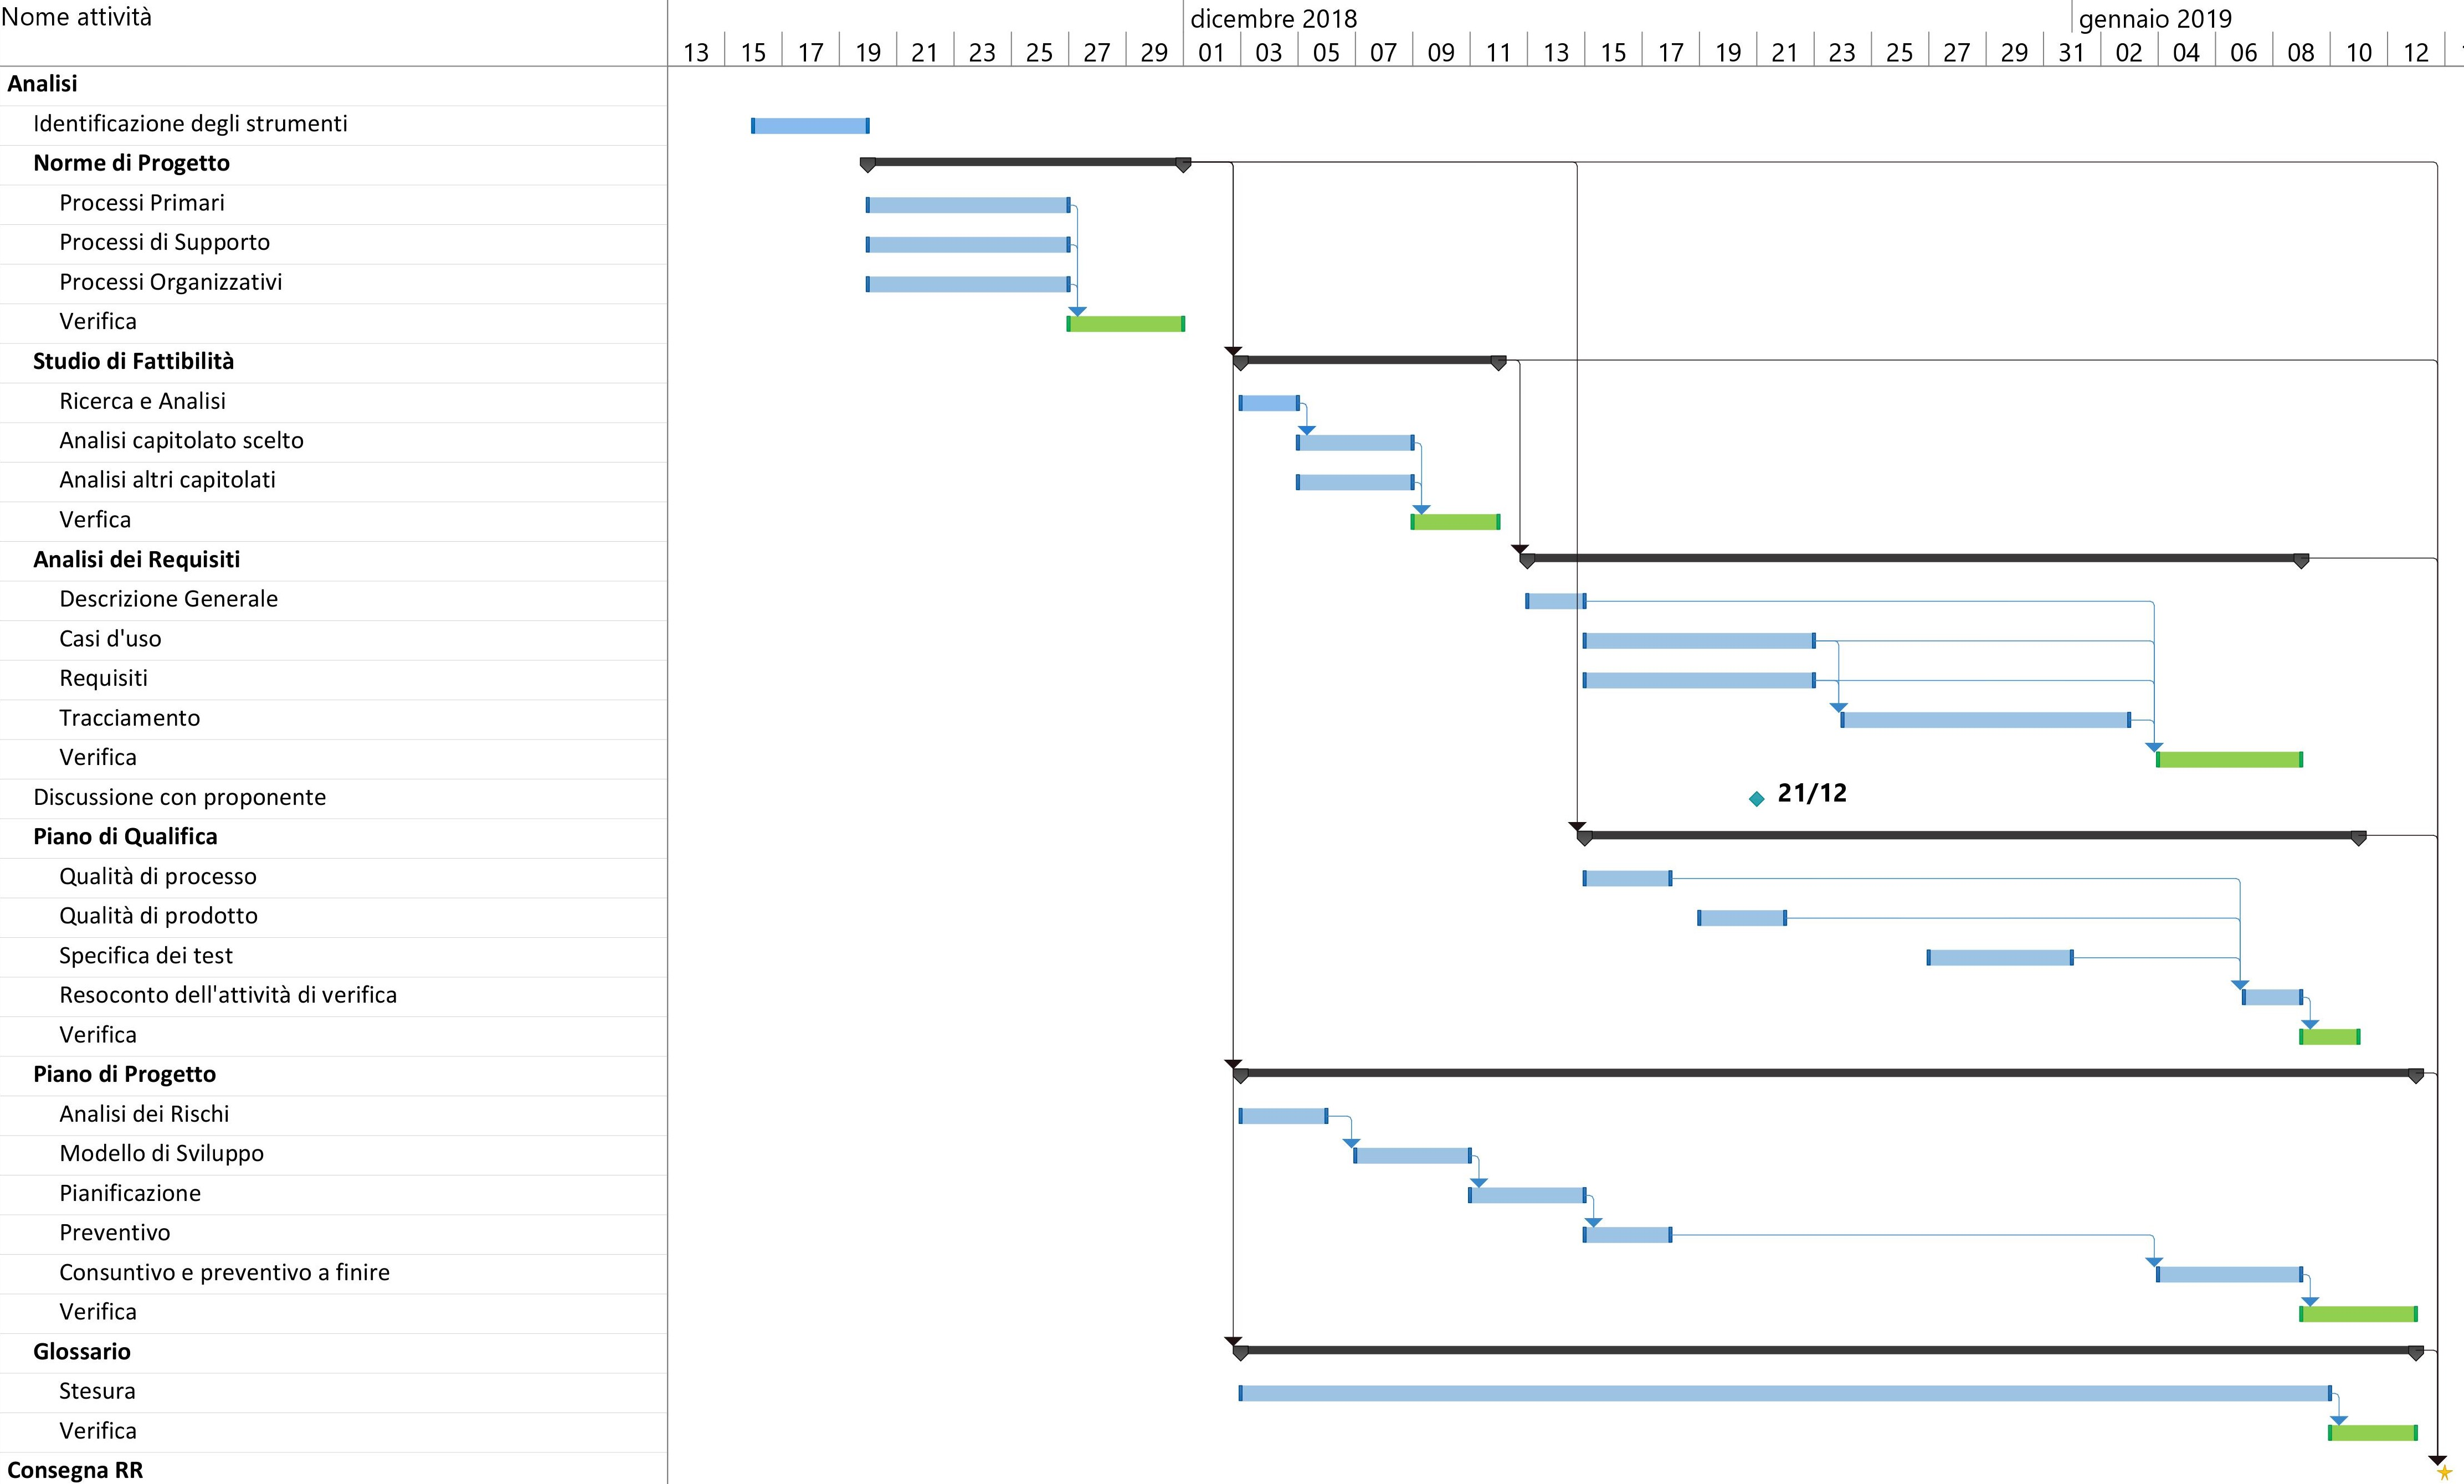
\includegraphics[width=0.99\linewidth]{res/images/gantt_analisi.jpg}
	\caption{Diagramma di Gantt della fase di Analisi}
\end{figure}


\subsection{Consolidamento dei requisiti}
\textit{Periodo: dal 2019-01-14 al 2019-01-21} \\
Questa fase comincia con la fine della fase di Analisi e termina il 
giorno della presentazione della Revisione dei Requisiti. Le attività 
di questa fase sono:
\begin{itemize}
	\item \textbf{Consolidamento}: questa attività ha lo scopo di consolidare e 
	migliorare i requisiti ottenuti nella fase precedente;
	\item \textbf{Preparazione alla presentazione}: durante questa attività 
	viene preparato il materiale necessario alla presentazione del 2019-01-21;
	\item \textbf{Incremento e verifica}: se necessario vengono migliorati i 
	documenti prodotti nella fase precedente;
	\item \textbf{Approfondimento personale}: ogni componente del gruppo dovrà 
	dedicare almeno 15 ore di studio e approfondimento delle tecnologie 
	necessarie alle prossime fasi e alla realizzazione del prodotto. Questa 
	attività verrà gestita in modo autonomo dai membri del gruppo, quindi non 
	sarà riportata nel diagramma di Gantt~\ref{fig:gantt_con} sottostante.
\end{itemize}

\begin{figure}[H]
	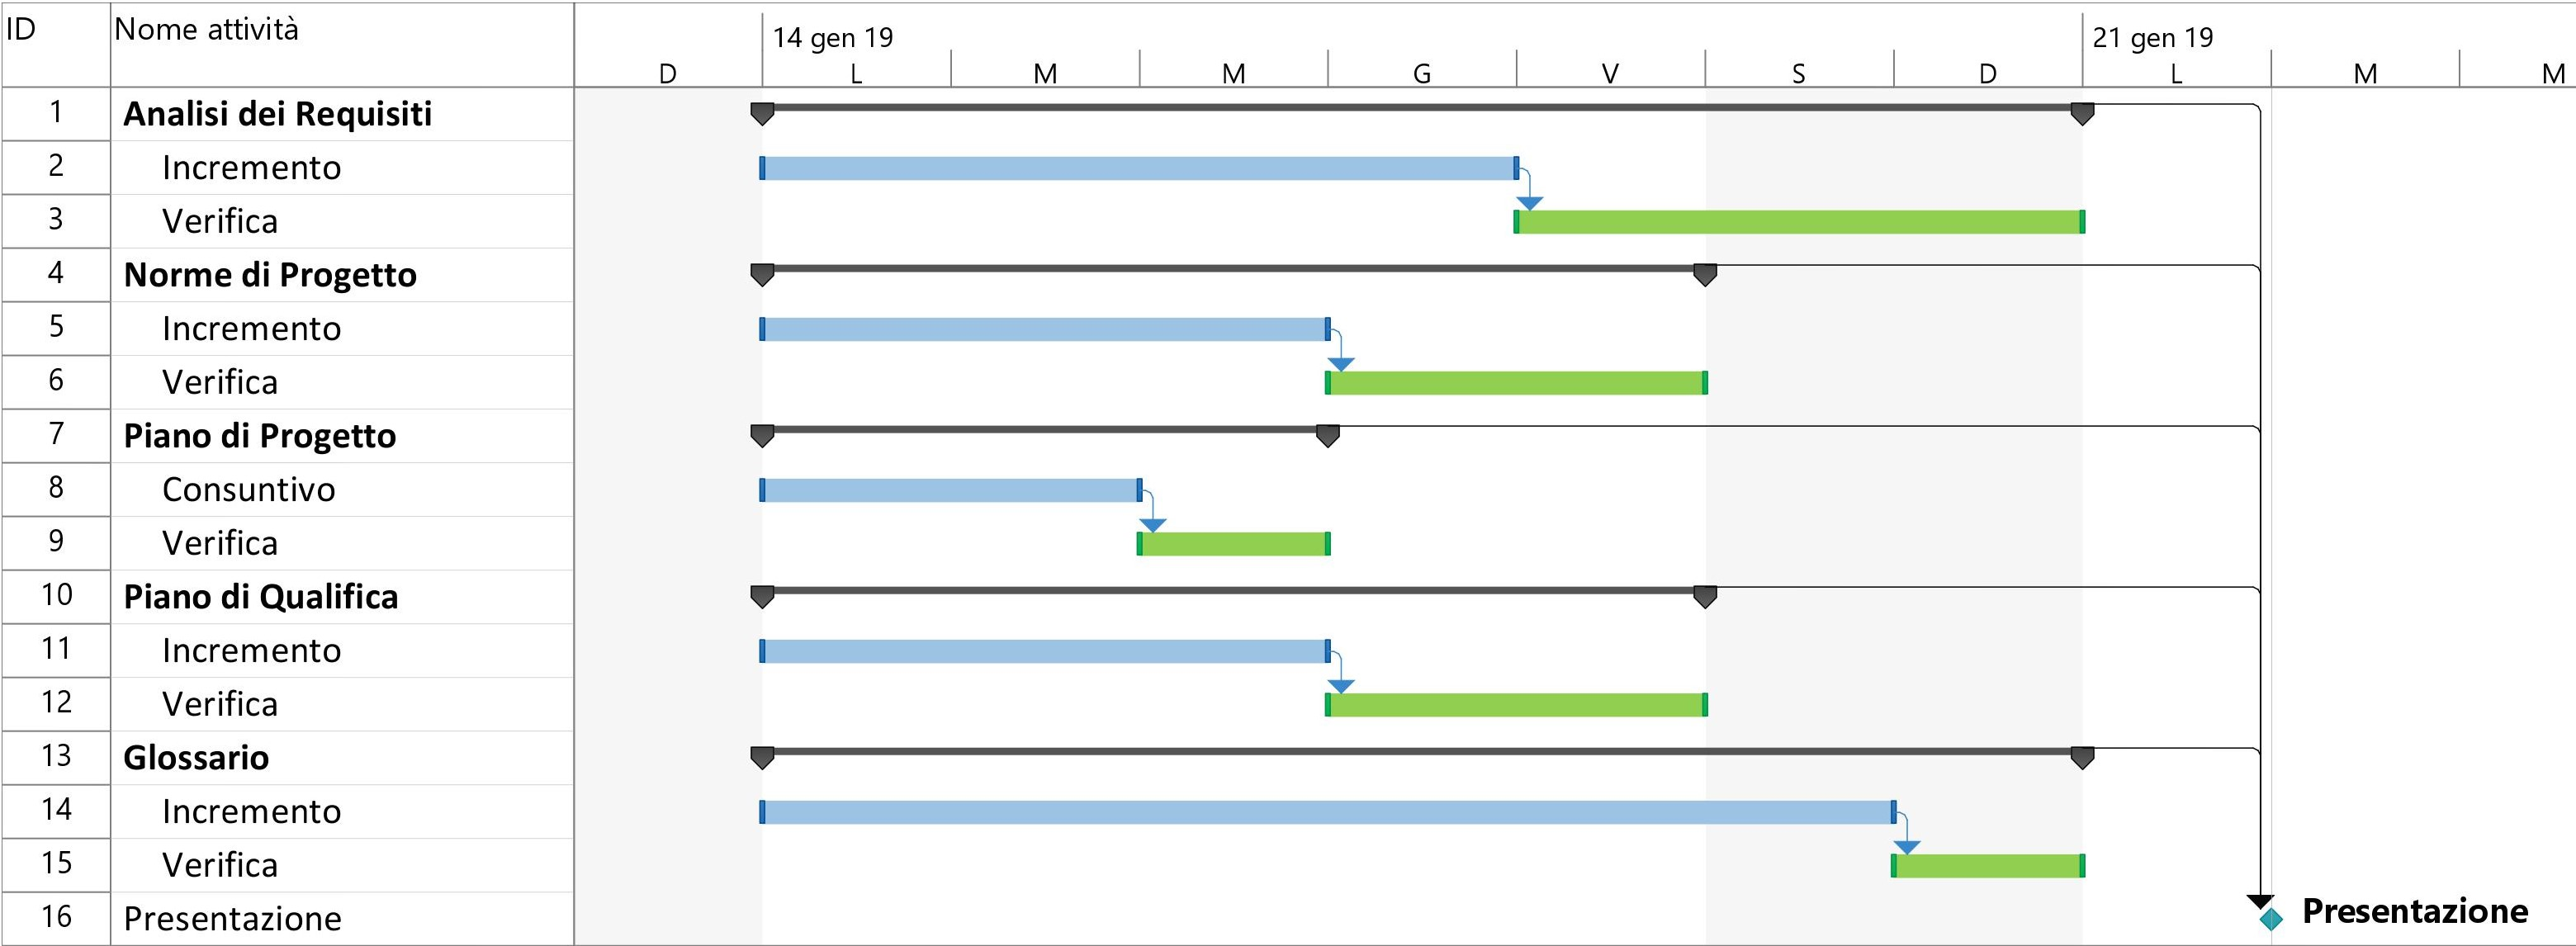
\includegraphics[width=0.99\linewidth]{res/images/gantt_cons.jpg}
	\caption{Diagramma di Gantt della fase di Consolidamento dei requisiti}
	\label{fig:gantt_con}
\end{figure}

%-----------------Sottosezione Progettazione Architetturale---------------------
\subsection{Progettazione architetturale}
\textit{Periodo: dal 2019-01-21 al 2019-03-08} \\
Questa fase comincia il giorno successivo alla presentazione e la fine coincide con la data di consegna Revisione di 
Progettazione. In questo periodo verrà individuata una soluzione architetturale 
tale per cui i requisiti richiesti vengano soddisfatti.
\begin{itemize}
	\item \textbf{Incremento e verifica}: se necessario vengono migliorati i documenti prodotti nelle fasi precedenti, con le modifiche e/o aggiunte pertinenti;
	\item \textbf{Technology Baseline}: %viene redatto l'Allegato Tecnico nel quale vengono individuati i design 
	%pattern\glosp che verranno adottati per lo sviluppo. Inoltre il documento 
%	include il tracciamento dei requisiti.\\
	viene codificato il \textbf{Proof of Concept}\glosp il quale viene presentato o condiviso tramite repository al committente e proponente in una data da definirsi. Tale prodotto è necessario per testare che tutte le tecnologie scelte riescano a soddisfare i requisiti individuati. In questo periodo saranno implementati solo una parte di requisiti, ovvero quelli che ricoprono le funzionalità di base. Successivamente verranno raffinati i requisiti già implementati, se non completi, e saranno implementate le funzionalità che permetteranno di soddisfare tutti i requisiti. \\
	Sono stati individuati degli incrementi per facilitare l'organizzazione del lavoro di codifica e gestire le dipendenze tra le funzionalità:
	\begin{itemize}
		\item \textbf{Incremento 1: Registrazione}: verrà implementata la registrazione alla piattaforma, mediante l'ausilio del plug-in\glosp MetaMask\glosp e degli smart contract\glo;
		\item \textbf{Incremento 2: Login}: verrà implementato il login, utilizzando le tecnologie sopra descritte;
		\item \textbf{Incremento 3: Home}: verrà implementata la home page del sito. Verranno usate le librerie React\glosp e Redux\glosp per gestire il front-end\glosp e verrà implementato il carrello per poter acquistare i beni e servizi offerti;
		\item \textbf{Incremento 4: Pagina Governo}: verranno implementate le funzionalità di coniazione e distribuzione dei Cubit\glo;
		\item \textbf{Incremento 5: Pagina Cittadino}: verranno implementati il pagamento in Cubit\glosp e la gestione degli ordini;
		\item \textbf{Incremento 6: Pagina Azienda}: verranno implementate alcune delle funzionalità riguardanti la gestione degli ordini e dell'IVA.
	\end{itemize}

\end{itemize}

\begin{figure}[H]
	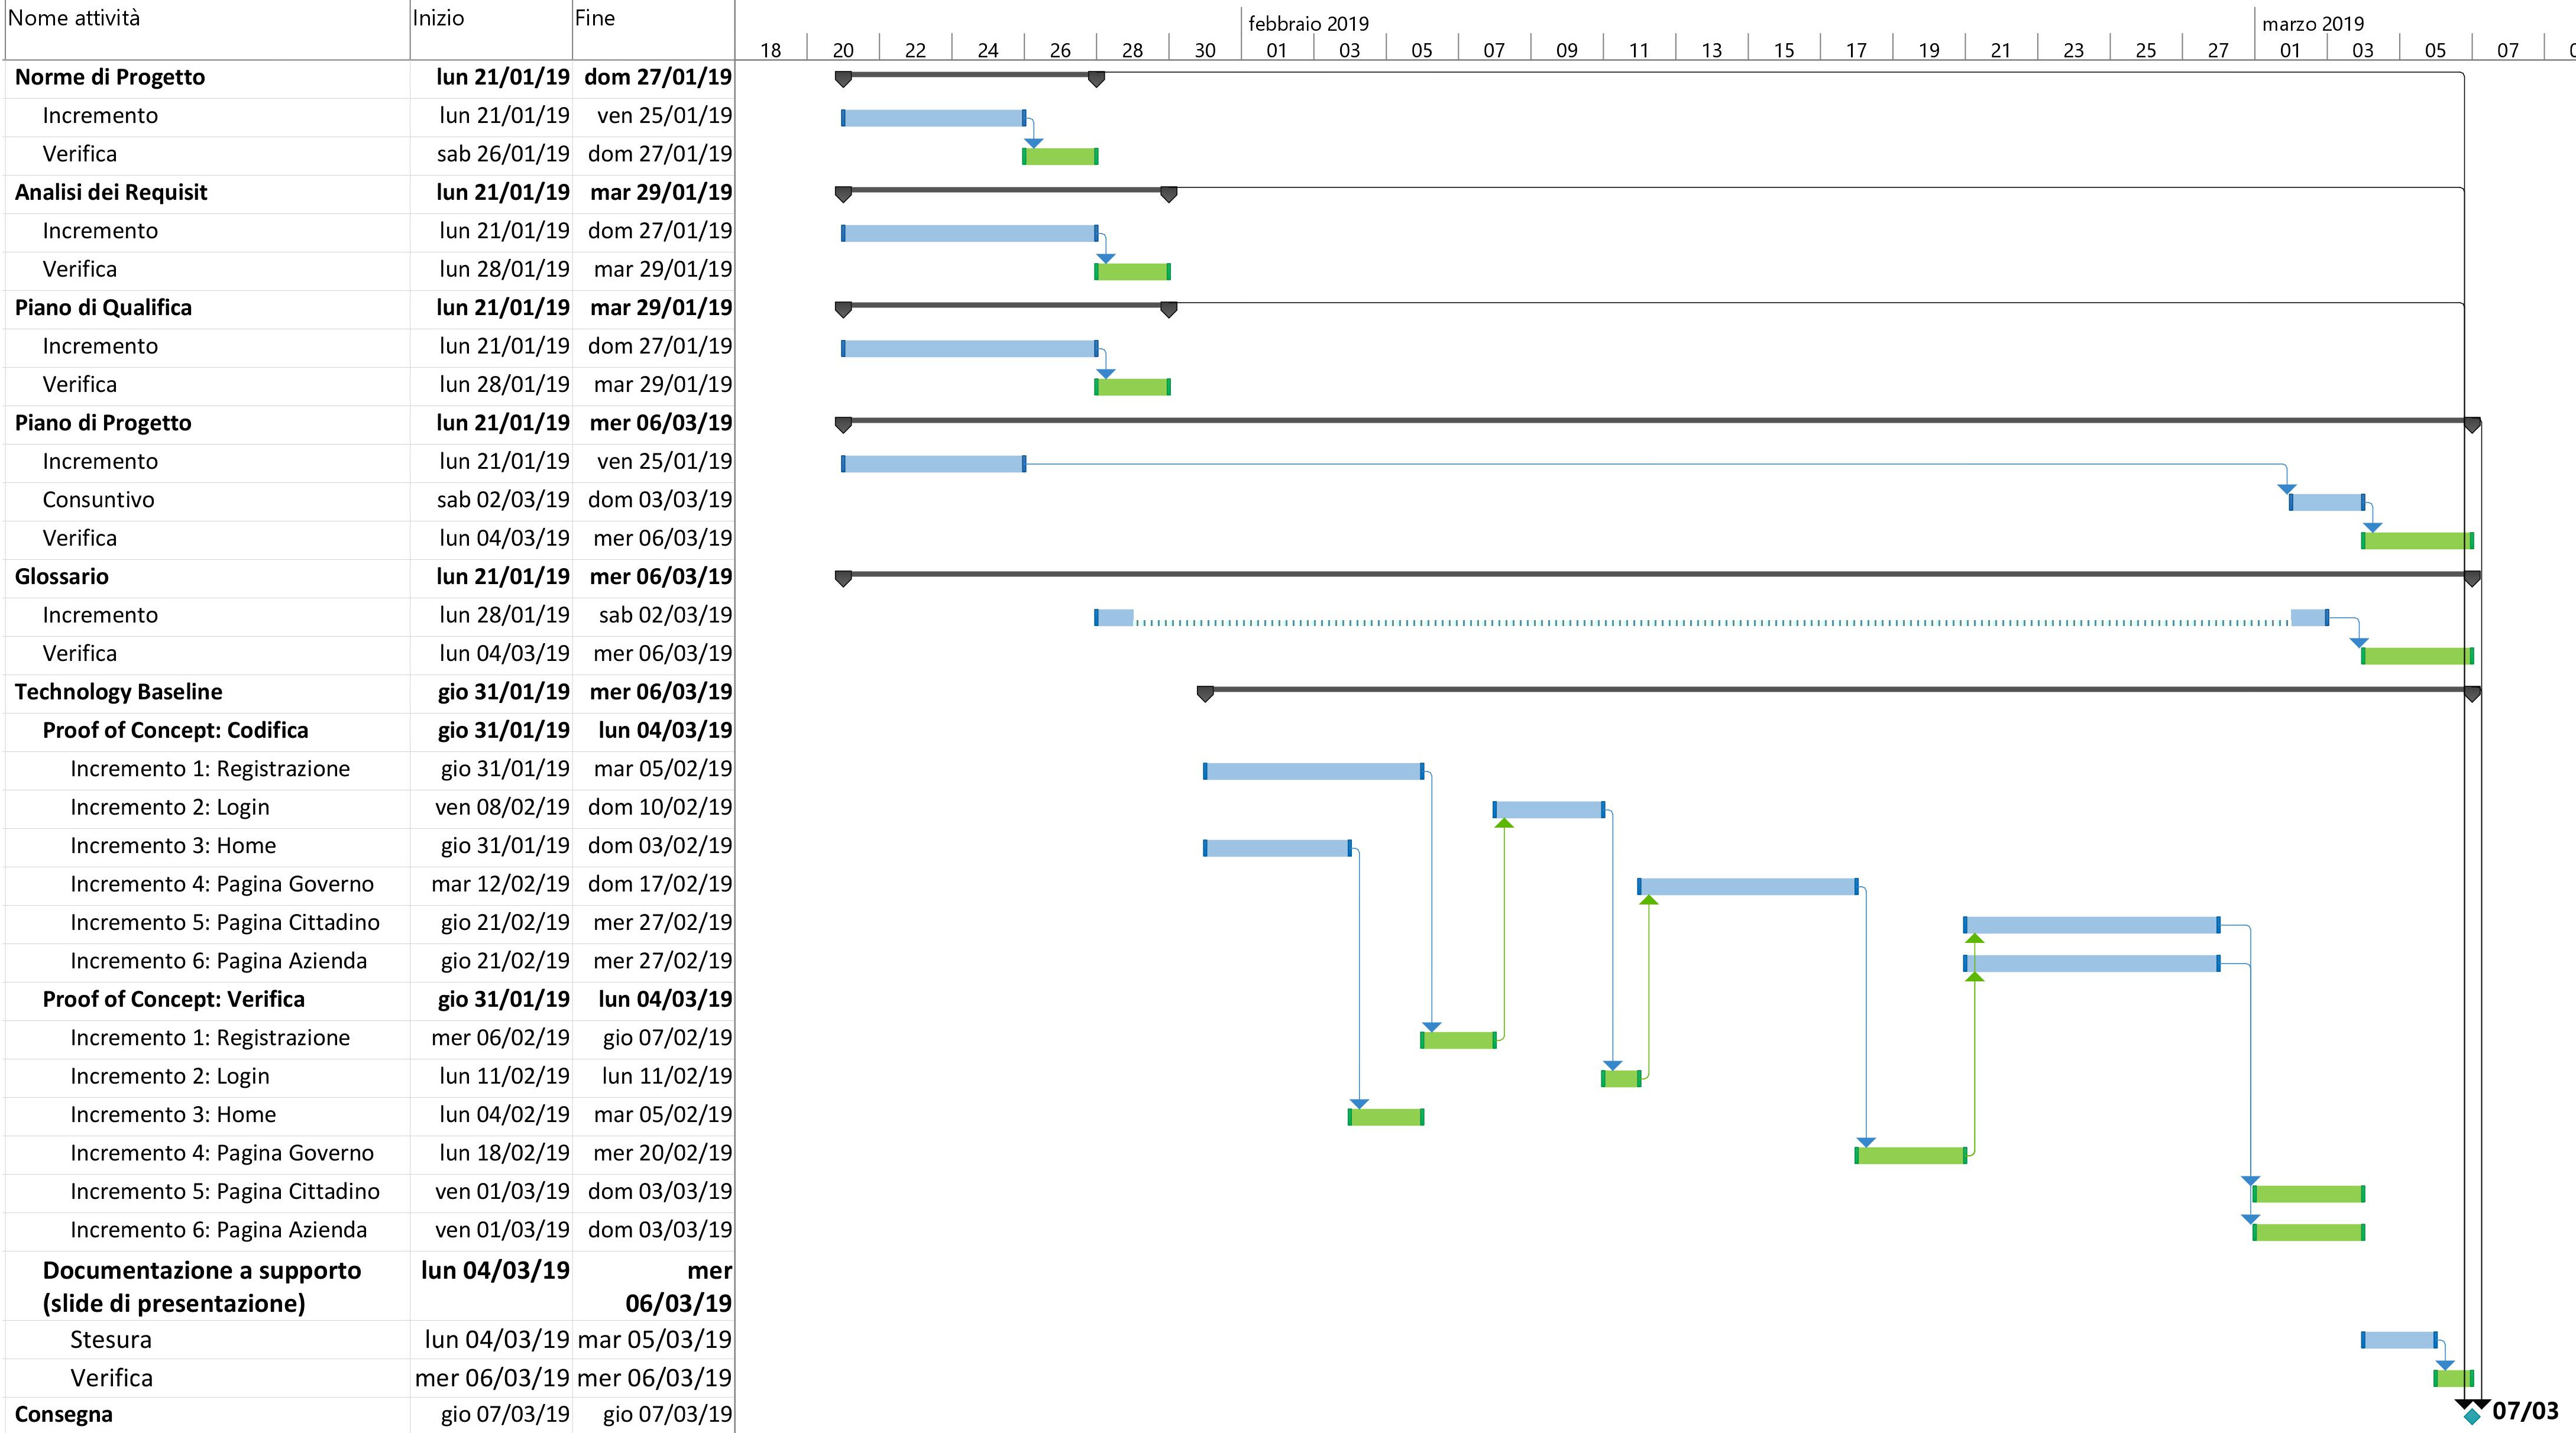
\includegraphics[width=0.99\linewidth]{res/images/gantt_pa.jpg}
	\caption{Diagramma di Gantt della fase di Progettazione architetturale}
\end{figure}


%-------------------Sottosezione Progettazione di Dettaglio---------------------
\subsection{Progettazione di dettaglio e codifica}
\textit{Periodo: dal 2019-03-15 al 2019-04-12} \\
L'inizio di questa fase è il giorno della scadenza della \textit{Revisione di 
Progettazione} e la data di fine coincide con la data di consegna dei documenti 
in vista della \textit{Revisione di Qualifica}. Le attività di questa fase sono:
\begin{itemize}
	\item \textbf{Product Baseline}: a seguito della \textit{Technology 
	Baseline} l'architettura individuata in essa viene scomposta nelle sue unità,
	che sono analizzate in profondità per fornire i 
	dettagli necessari alla loro codifica e verifica. A supporto 
	di ciò viene redatto l'Allegato Tecnico di supporto alla Product Baseline;
	\item \textbf{Codifica}: questa attività consiste nella scrittura del 
	codice e della sua verifica con modalità e strumenti definiti nel 
	\textit{Piano di Qualifica v2.0.0}
	\item \textbf{Manuale Utente}: viene redatto il documento \textit{Manuale 
	Utente} atto a fornire istruzioni e indicazioni per l'utilizzo del prodotto;
	\item \textbf{Incremento e verifica}: se necessario vengono migliorati i 
	documenti prodotti nelle fasi precedenti.
\end{itemize}

\begin{figure}[H]
	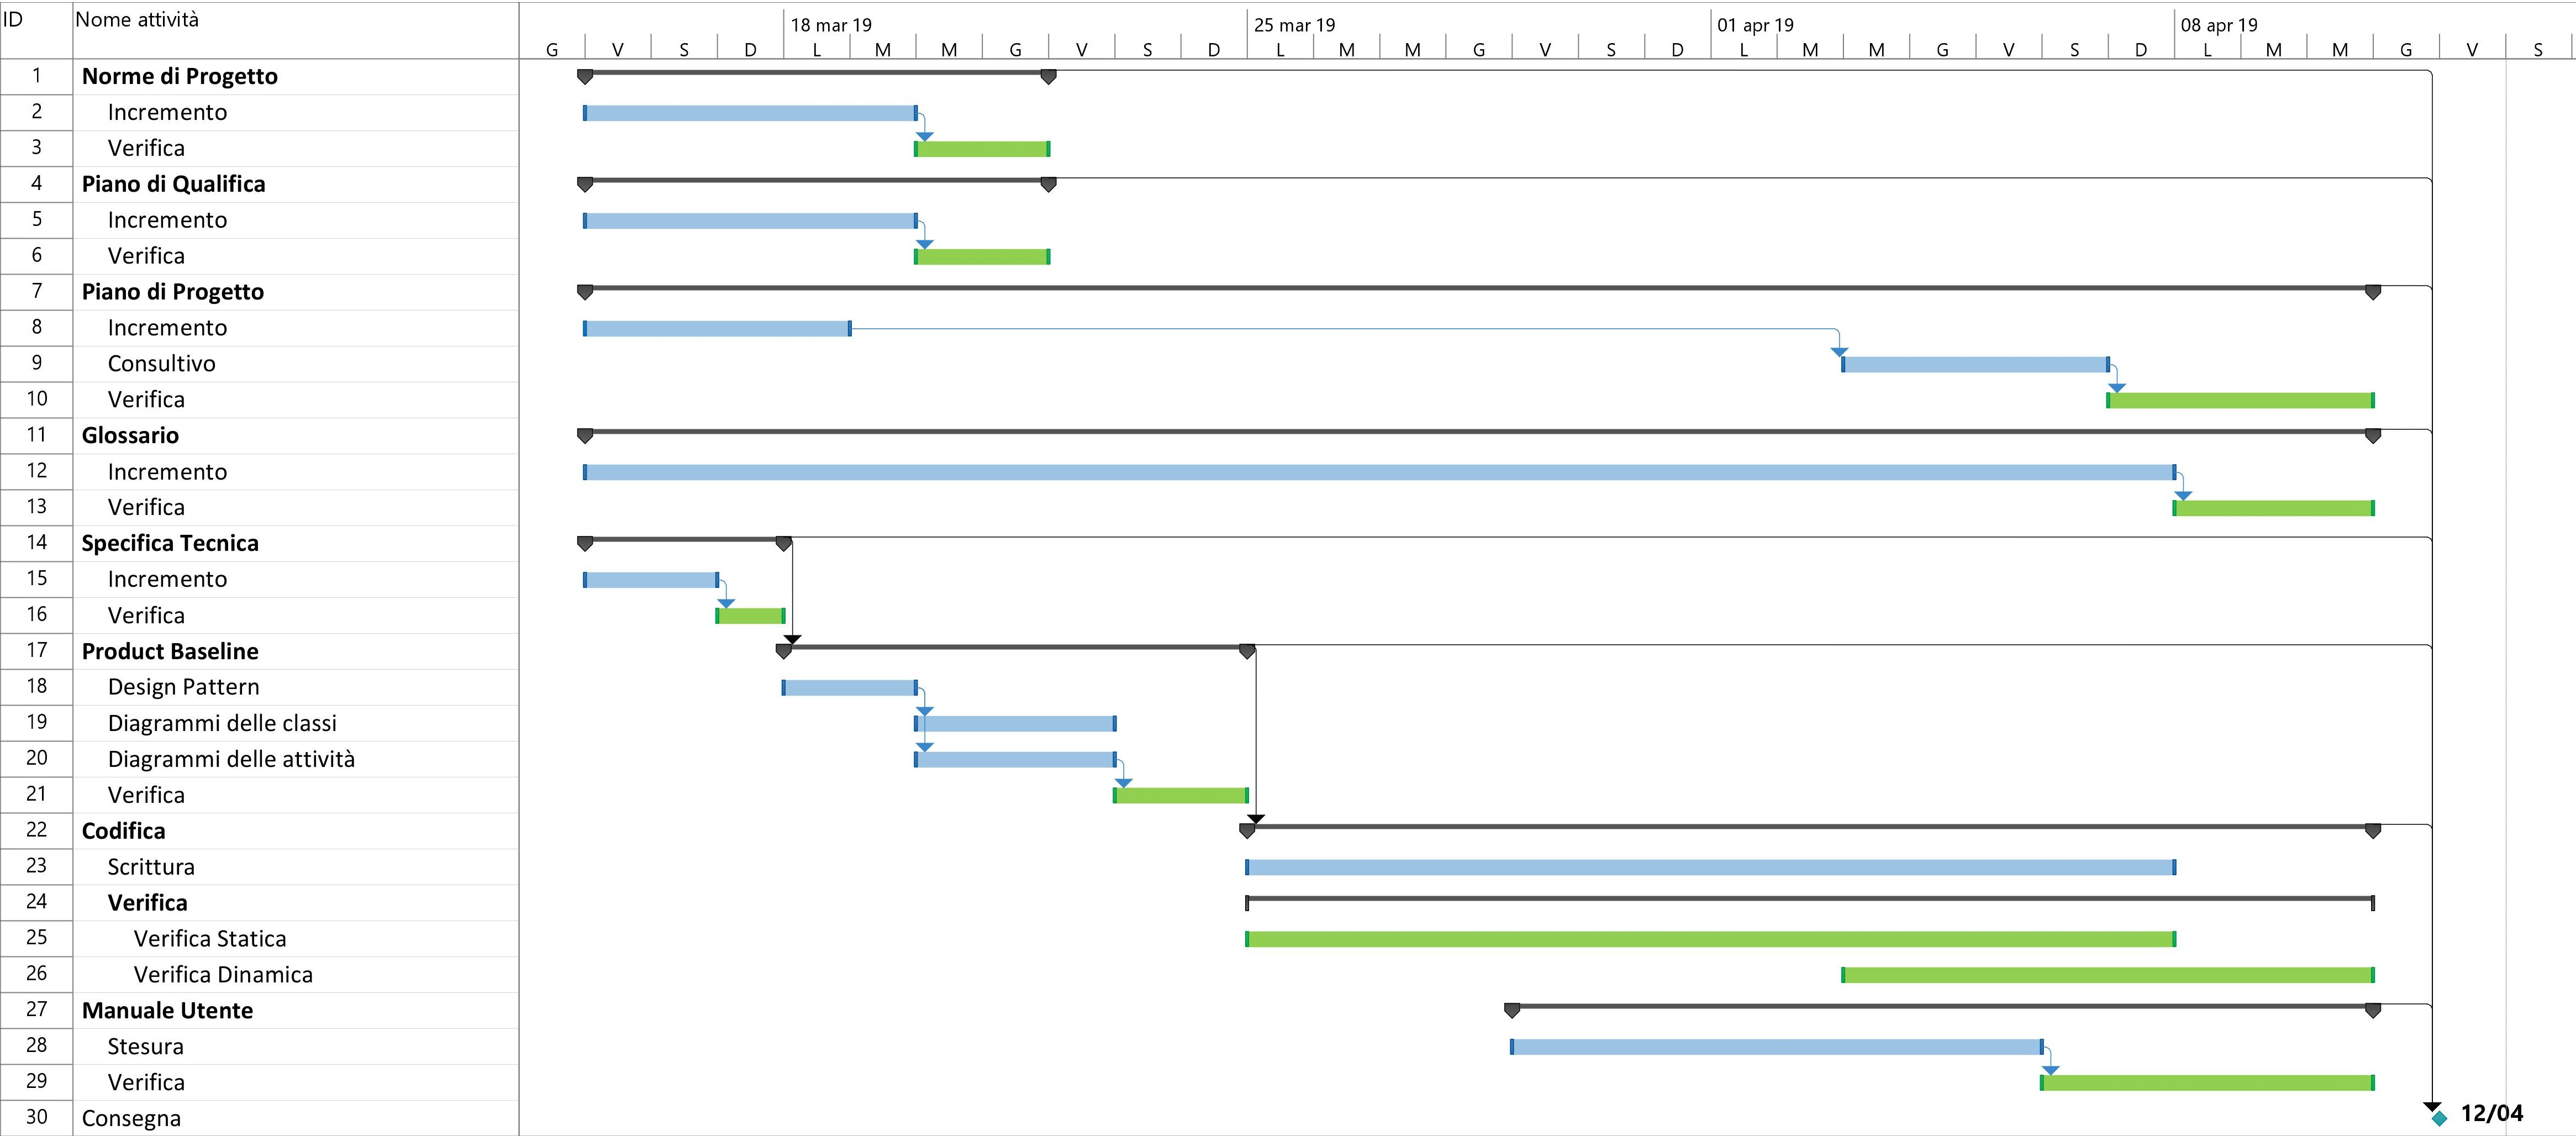
\includegraphics[width=0.99\linewidth]{res/images/gantt_pd.jpg}
	\caption{Diagramma di Gantt della fase di Progettazione di dettaglio e codifica}
\end{figure}
\pagebreak


\subsection{Validazione e collaudo}
\textit{Periodo: dal 2019-04-12 al 2019-05-17 } \\
L'inizio di questa fase coincide con la data di consegna dei documenti per la 
\textit{Revisione di Qualifica}, mentre la data di fine coincide con la 
consegna in vista della \textit{Revisione di Accettazione}. Durante questo periodo 
si eseguiranno ulteriori attività di validazione e verifica. Le attività 
previste sono: 
\begin{itemize}
	\item \textbf{Validazione e collaudo}: per la parte di collaudo si 
	eseguiranno ulteriori test sul prodotto, in modo da garantirne la 
	correttezza e stabilità. Per la parte di validazione, verrà 
	valutata la coerenza del prodotto e dei requisiti specificati nel documento 
	\textit{Analisi dei Requisiti} nella sua ultima versione;
	\item \textbf{Manuale Sviluppatore}: viene redatto il documento \textit{Manuale Sviluppatore} atto a fornire tutte le informazioni necessarie al mantenimento, manutenzione e ampliamento del prodotto finale;
	\item \textbf{Incremento e verifica}: se necessario vengono migliorati i 
	documenti prodotti nelle fasi precedenti.
\end{itemize}
\begin{figure}[H]
	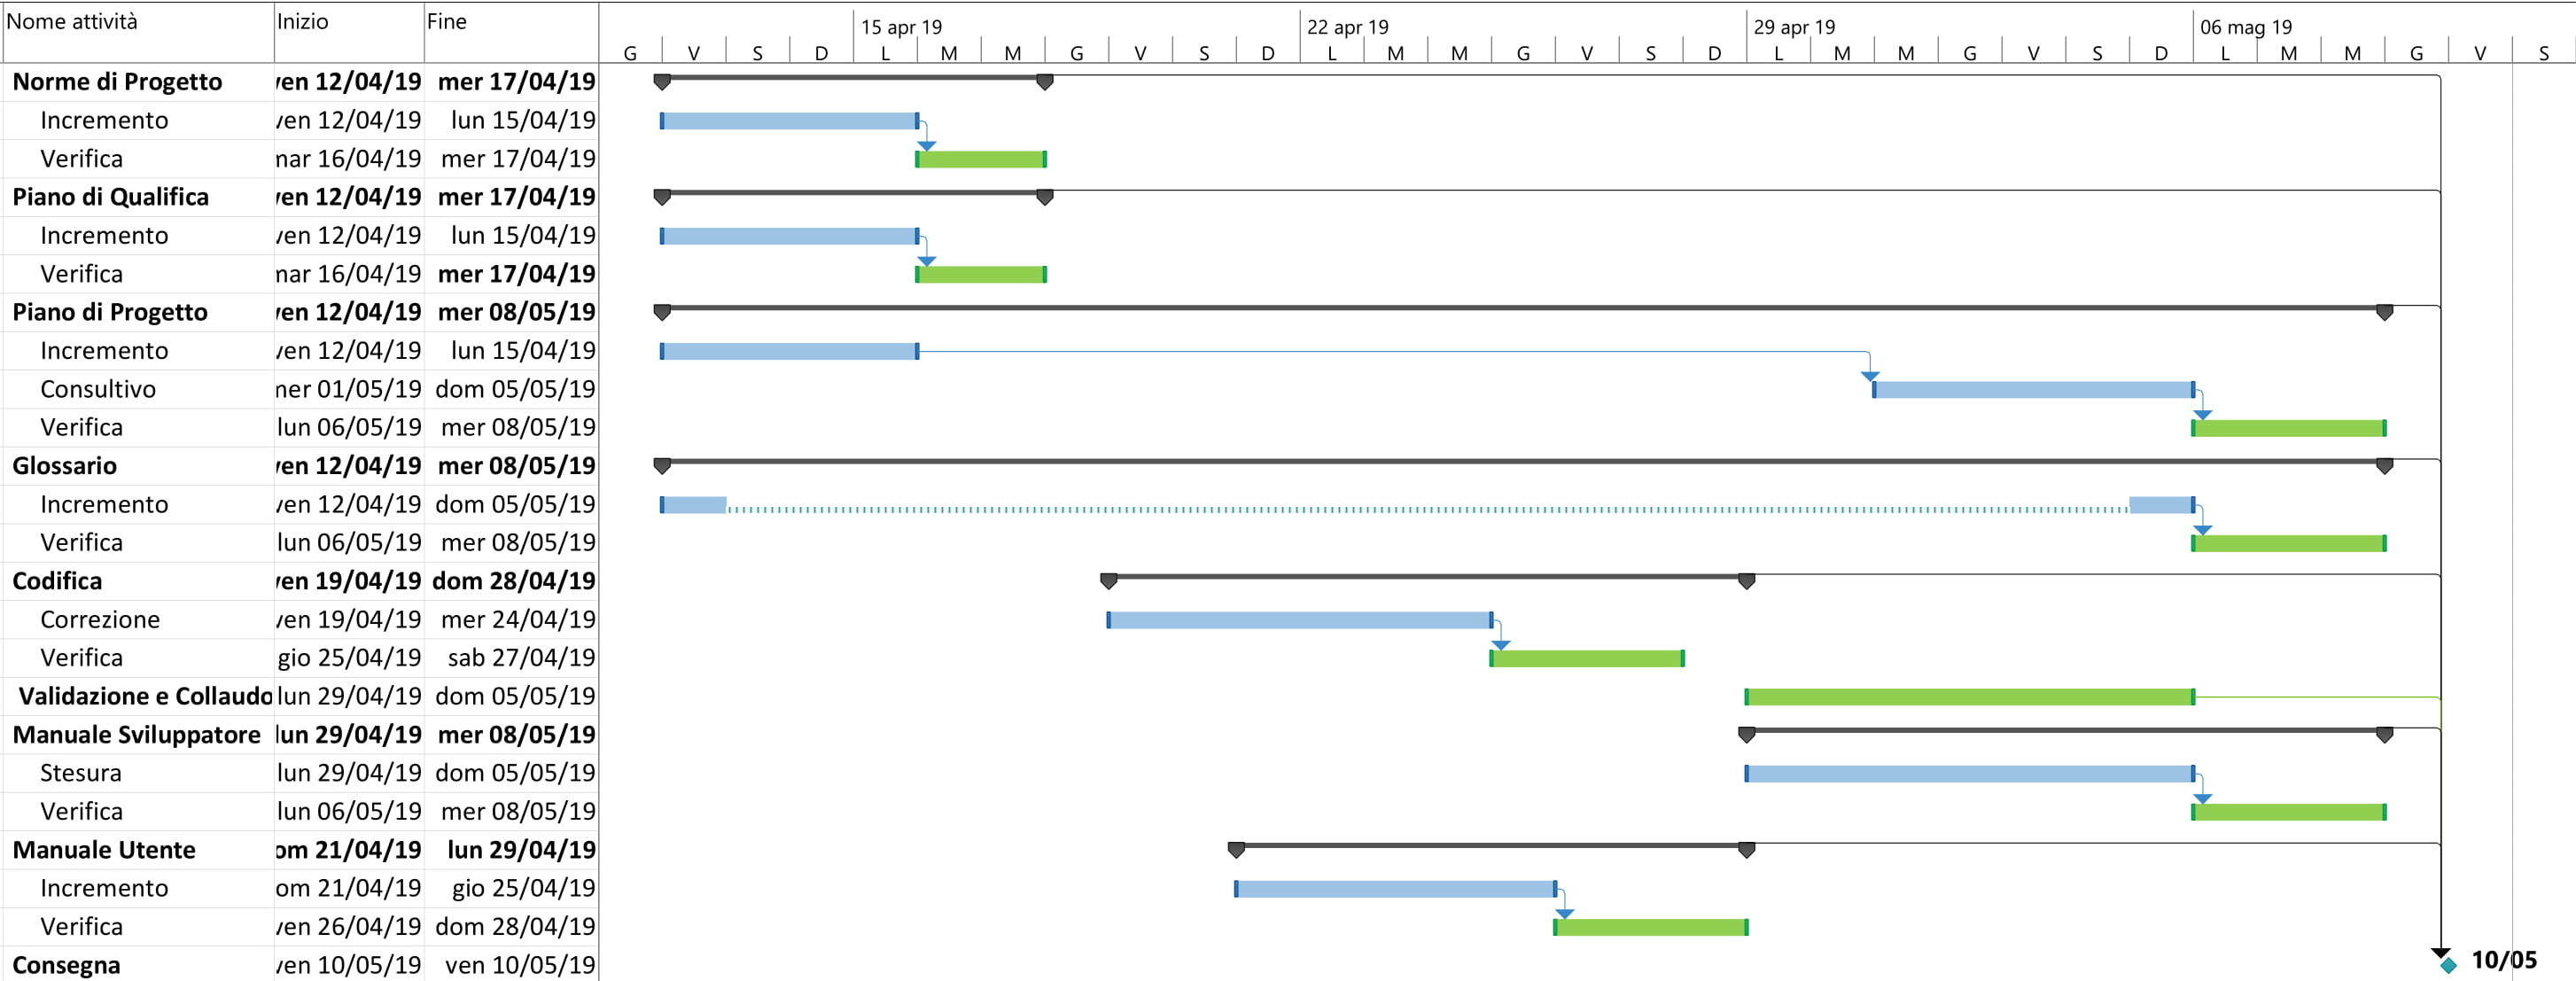
\includegraphics[width=0.99\linewidth]{res/images/gantt_val.jpg}
	\caption{Diagramma di Gantt della fase di validazione e collaudo}
\end{figure}